\definecolor{salmon}{RGB}{255,191,191}
\definecolor{leak}{RGB}{255,151,117}
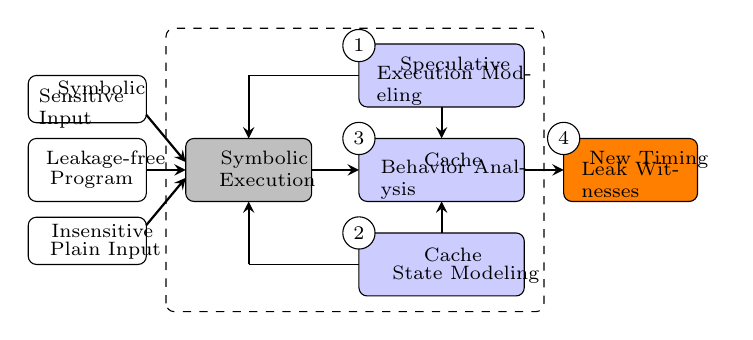
\begin{tikzpicture}[fill=blue!20,font=\scriptsize] 
  \tikzstyle{arrow}=[thick,->,>=stealth,black]
  \tikzstyle{txt}=[above=5pt,right,text width=1.6cm]
  \tikzstyle{long_txt}=[above=5pt,right,text width=2cm]
  \tikzstyle{short_txt}=[above=5pt,right,text width=1.4cm]

  % blocks on left    			
  \draw [rounded corners=3] (0.0, 2.2) rectangle (1.5, 2.8);
  \node [above=5pt,right,text width=1.6cm] at (0.25, 2.45) {Symbolic};
  \node [above=5pt,right,text width=1.6cm] at (0.01, 2.2) {Sensitive Input};

  \draw [rounded corners=3] (0.0, 1.2) rectangle (1.5, 2.0);
  \node [above=5pt,right,text width=1.6cm] at (0.1, 1.55) {Leakage-free};
  \node [above=5pt,right,text width=1.6cm] at (0.15, 1.3) {Program $\prog$};

  \draw [rounded corners=3] (0.0, 0.4) rectangle (1.5, 1.0);
  \node [above=5pt,right,text width=1.6cm] at (0.17, 0.65) {Insensitive};
  \node [above=5pt,right,text width=1.6cm] at (0.15, 0.4) {Plain Input};

  % line connecting first column and second column
  \draw [arrow](1.5, 2.3)--(2.0, 1.7);
  \draw [arrow](1.5, 1.6)--(2.0, 1.6);
  \draw [arrow](1.5, 0.9)--(2.0, 1.5);
  

  % blocks in the second column
  \draw [fill=lightgray, rounded corners=3] (2.0, 1.2) rectangle (3.6, 2.0);
  \node [txt] at (2.32,1.55){Symbolic};
  \node [txt] at (2.3,1.3){Execution};

  % blocks in the third column
  \draw [fill=blue!20, rounded corners=3] (4.2, 0) rectangle (6.3, 0.8);
  \node [txt] at (4.9,0.35){Cache};
  \node [long_txt] at (4.5,0.1){State Modeling};
  \draw [arrow] (2.8,0.4)--(2.8,1.2);
  \draw (2.8,0.4)--(4.2,0.4);
  
  \draw [fill=blue!20, rounded corners=3](4.2, 1.2) rectangle (6.3, 2.0);
  \node [txt] at (4.9,1.55){Cache};
  \node [long_txt] at (4.35,1.3){Behavior Analysis};
  \draw [arrow](5.25,0.8)--(5.25,1.2);
  \draw [arrow](3.6,1.6)--(4.2,1.6);

  \draw [fill=blue!20, rounded corners=3] (4.2, 2.4) rectangle (6.3, 3.2);
  \node [txt] at (4.6, 2.75) {Speculative};
  \node [long_txt] at (4.3, 2.5) {Execution Modeling};
  \draw [arrow](2.8, 2.8)--(2.8, 2.0);
  \draw (2.8, 2.8)--(4.2, 2.8);
  \draw [arrow] (5.25, 2.4)--(5.25, 2.0);

  % line connecting first column and second column
  \draw [arrow](6.3,1.6)--(6.8,1.6);

  % The fourth column
  \draw [fill=orange, rounded corners=3](6.8, 1.2) rectangle (8.5, 2.0);
  \node [txt] at (7,1.55){New Timing};
  \node [txt] at (6.9,1.3){Leak Witnesses};

  % the dashed rectangle
  \draw [dashed,black,thin,rounded corners=3](1.75, -0.2) rectangle (6.55, 3.4);

  % the numbers
  \node [draw,circle,fill=white,minimum size=2pt,inner sep=2pt] at (4.2,3.18) {1};
  \node [draw,circle,fill=white,minimum size=2pt,inner sep=2pt] at (4.2,0.8) {2};
  \node [draw,circle,fill=white,minimum size=2pt,inner sep=2pt] at (4.2,2.0) {3};
  \node [draw,circle,fill=white,minimum size=2pt,inner sep=2pt] at (6.8,2.0) {4};

\end{tikzpicture}

